\documentclass[hidelinks,12pt]{article}

\usepackage{amsmath}    % need for subequations
\usepackage{graphicx}   % need for figures
\usepackage{verbatim}   % useful for program listings
\usepackage{color}      % use if color is used in text
\usepackage{subfigure}  % use for side-by-side figures
\usepackage{hyperref}   % use for hypertext links, including those to external documents and URLs

\usepackage[numbered]{matlab-prettifier} % including matlab w/ syntax highlighting
\usepackage[T1]{fontenc} % prettier matlab font
\lstMakeShortInline[style=Matlab-editor]| % matlab inline escape character

\usepackage[
top    = 2.75cm,
bottom = 2.50cm,
left   = 3.00cm,
right  = 2.50cm]{geometry}

\graphicspath{ {./Figures/} }

% don't need the following. simply use defaults
\setlength{\baselineskip}{16.0pt}    % 16 pt usual spacing between lines



\begin{document}
\pagenumbering{gobble}
\begin{center}
  {\huge Homework 5}\\
  \vspace{10px}
  
\includegraphics{Logo} \\
  Date of Submission:\\
  February 25, 2019\\
  \vspace{30px}
  \rule{300px}{0.5px} \\
  Thorne Wolfenbarger \\
  \href{mailto:wolfent1@my.erau.edu}{wolfent1@my.erau.edu} \\
  \vspace{30px}
  Submitted to: \\
  Professor Kaela Martin \\
  College of Engineering \\
  \vspace{40px}
  In Partial Fulfillment \\
  of the Requirements of \\
  \vspace{10px}
  AE 313 \\
  Space Mechanics \\
  Spring, 2019 \\
\end{center}

\pagenumbering{arabic}
\begin{center}
\large AE 313 Homework 10
\end{center}
\flushleft
1. Draw the Jupiter-centered vector diagram of the fly-by.\\
\begin{figure}[!htb]
  \center
  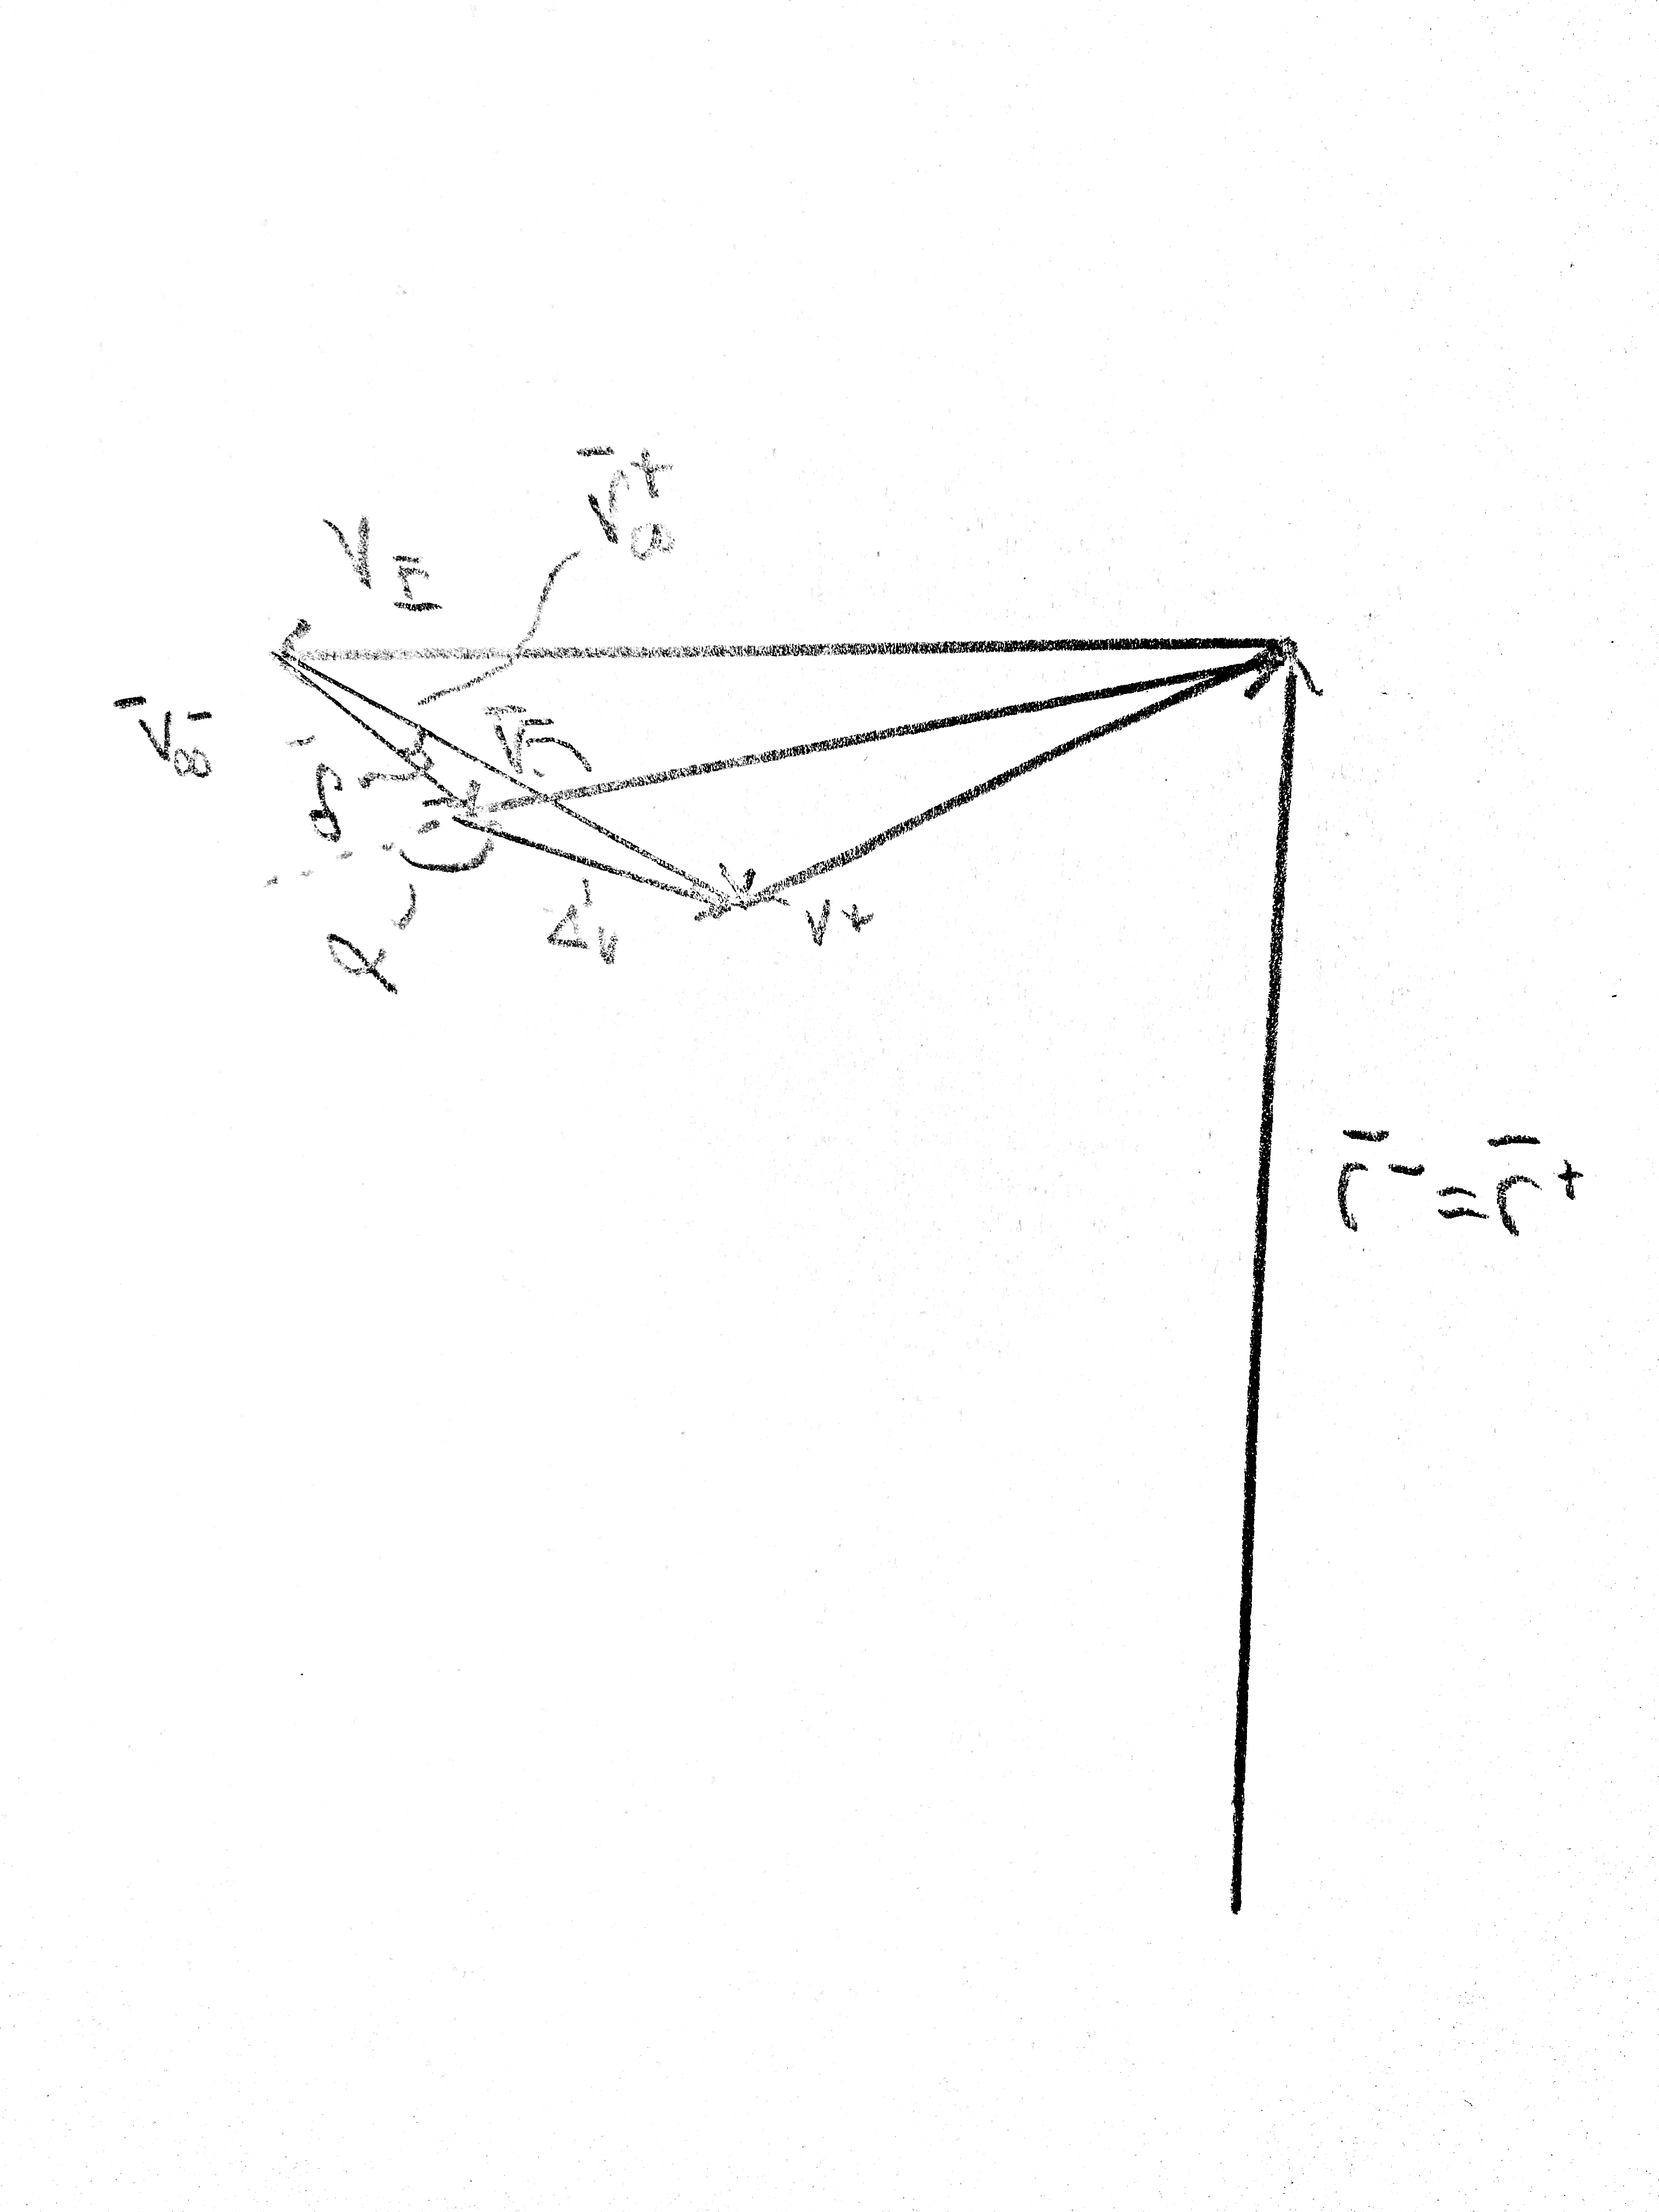
\includegraphics[scale=0.1]{1}
  \caption{Fly-by diagram}
  \label{fig:Fig01}
\end{figure}
\vspace{10px}
2. Find $\theta^{^*-}$\\
\begin{lstlisting}[frame=lines,style=Matlab-editor,basicstyle = \mlttfamily]
ta_clipper1m = atan2d( r_clipper1*v_clipper1m^2/MU('Jupiter') * cosd(FPA_clipper1m)*sind(FPA_clipper1m),...
    r_clipper1*v_clipper1m^2/MU('Jupiter') * cosd(FPA_clipper1m) - 1);
\end{lstlisting}
$\theta^{^*-}=-12.3219^\circ$\\
This angle is correct due to use of atan2. It is negative because the orbit is descending.
\vspace{10px}
\newpage
3. Determine the following: $r_{p/europa}, \alpha$\\
\begin{lstlisting}[frame=lines,style=Matlab-editor,basicstyle = \mlttfamily]
periapsis_europa = a_europa*(1-e_europa);
...
alpha = -alpha;
\end{lstlisting}
\begin{tabular}{ll}
$r_{p/europa \rightarrow clipper}=$&$1.3594 \cdot 10^3~km$\\
$\alpha=$&$-116.1968^\circ$\\
\end{tabular}\\
$\alpha$ is negative due to the problem statement.
\vspace{10px}
4. Does the spacecraft gain or lose energy? Why?\\
Geometrically, the spacecraft must lose energy. Observing `delta` it can be determined that the spacecraft must have lost energy since `delta` directs the dv vector opposing the initial velocity\\
\vspace{10px}
5. Does the spacecraft pass "ahead" or "behind"? Prove it with drawings. (Hint: Draw behind pass vs. ahead pass. How does $v_{inf}$ change?)\\
\begin{figure}[!htb]
  \center
  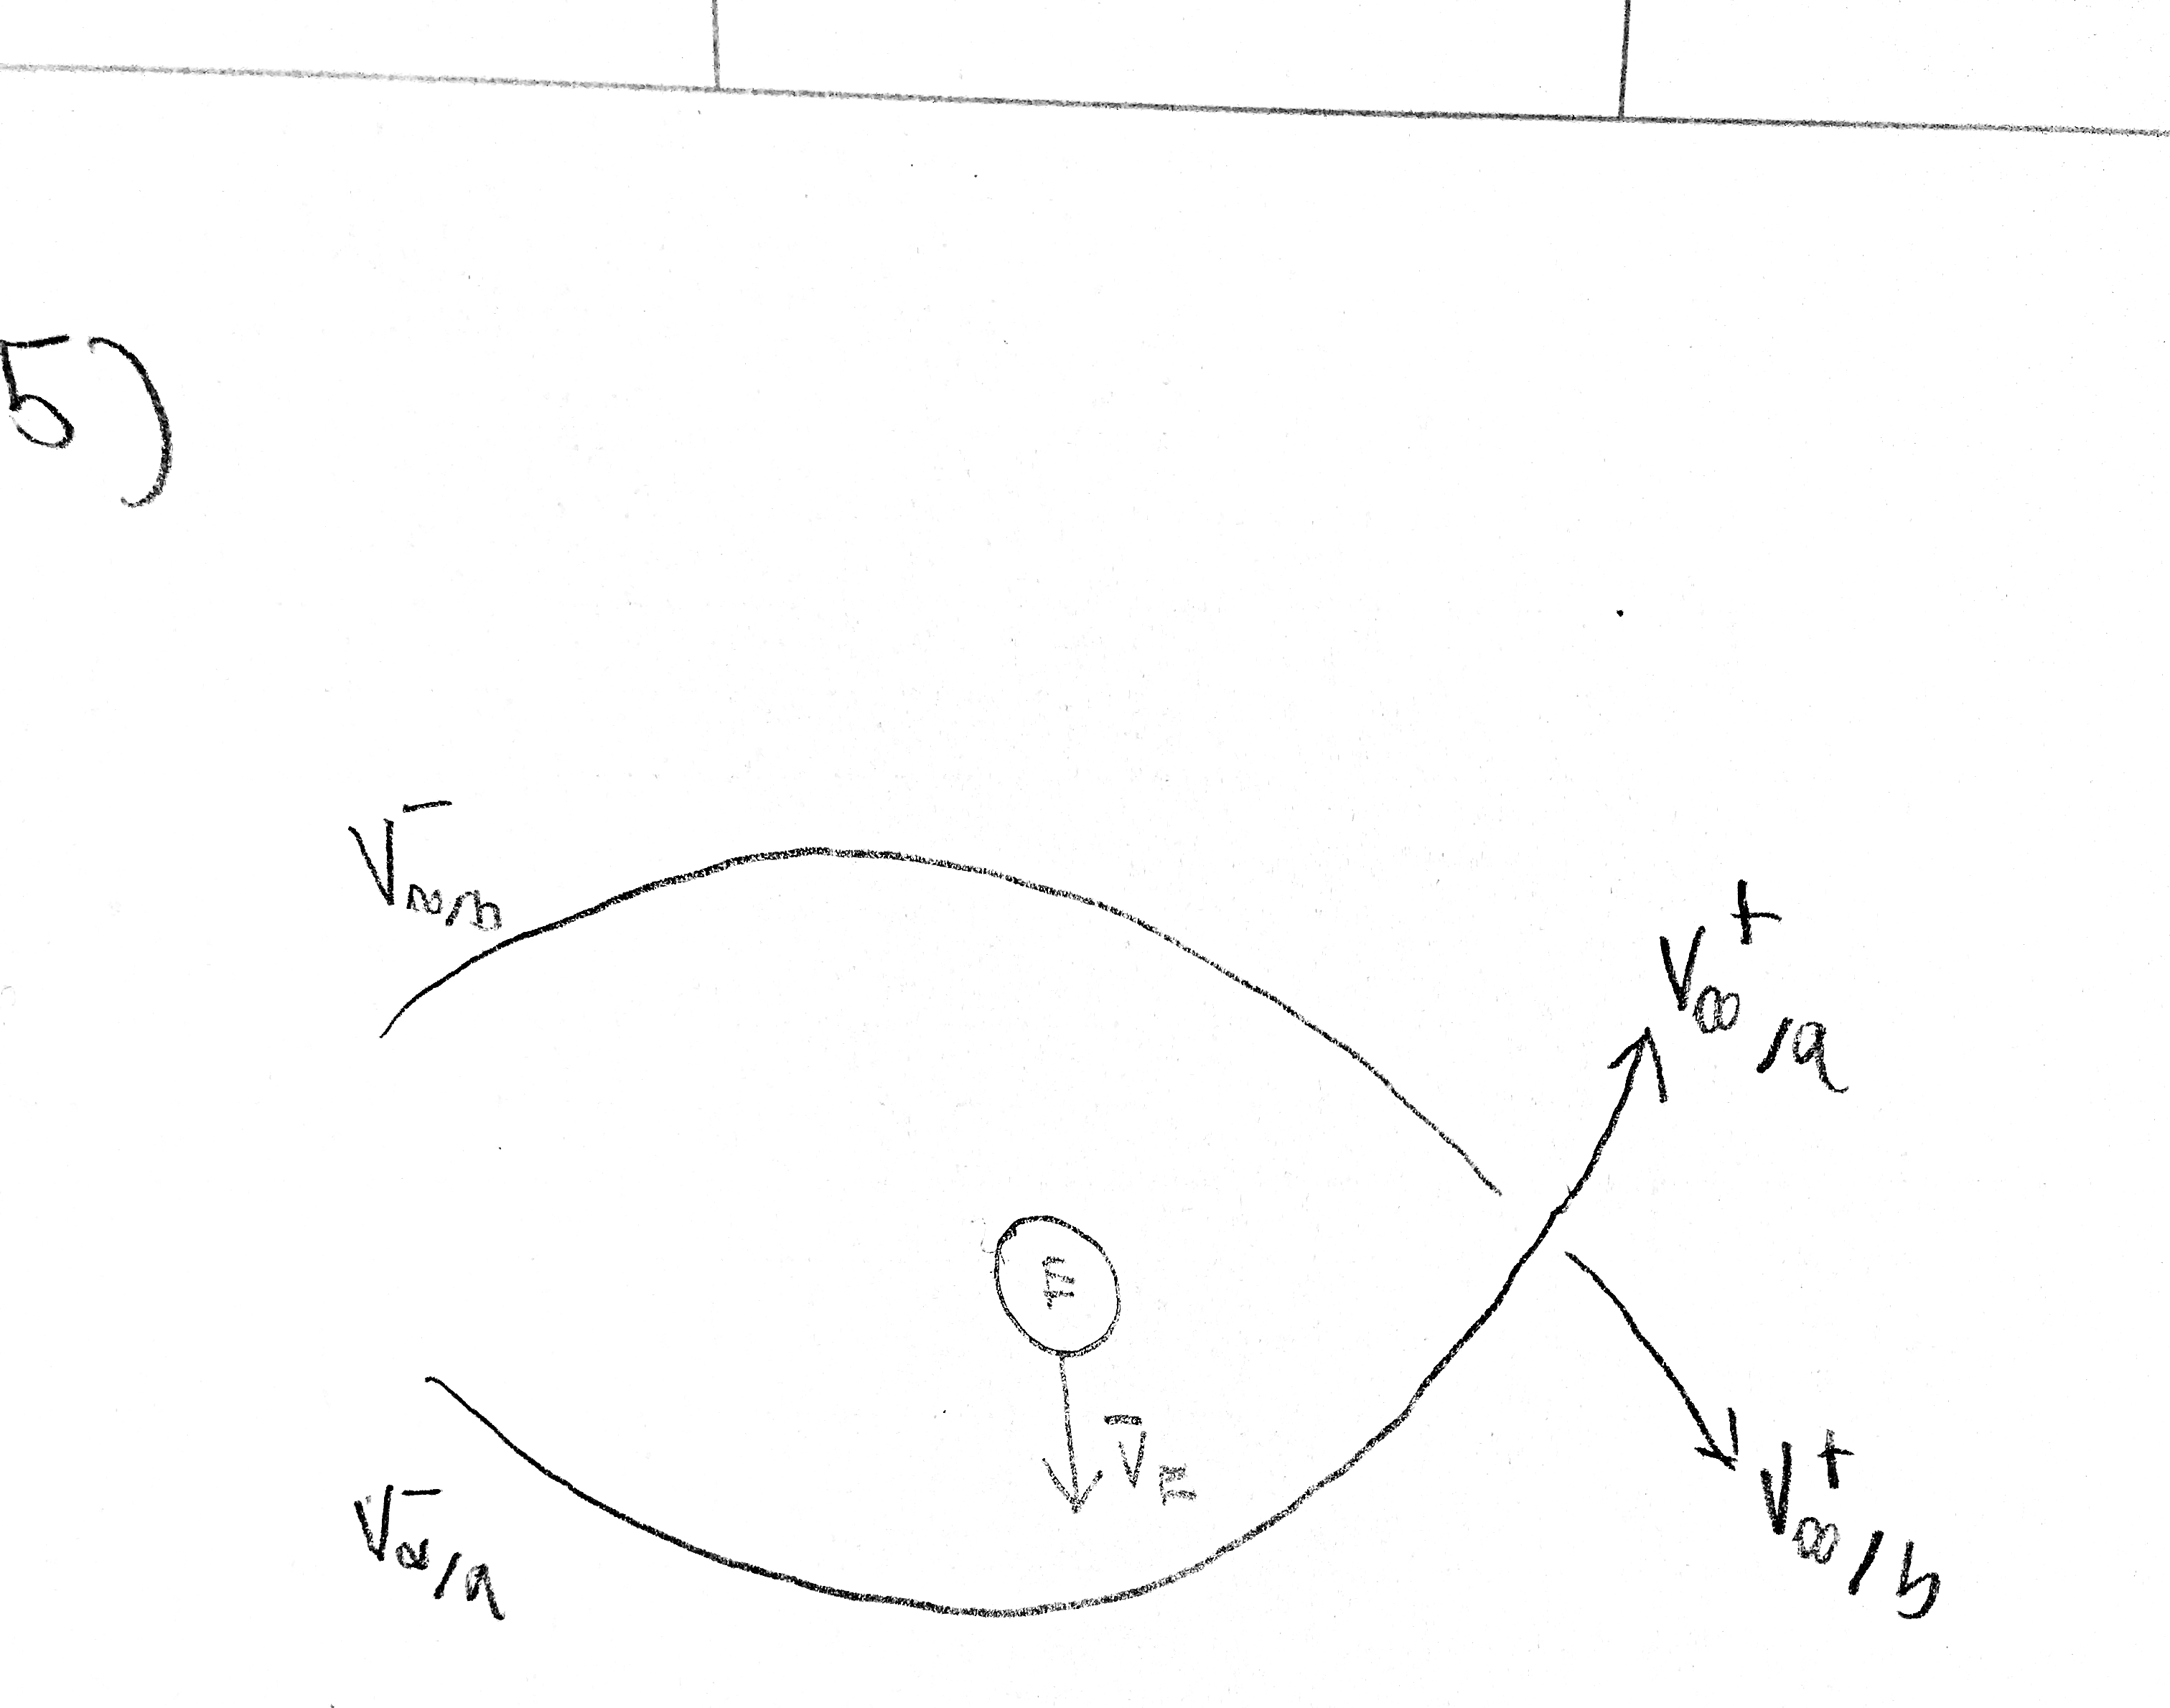
\includegraphics[scale=0.1]{5}
  \caption{Infinite Diagram}
  \label{fig:Fig02}
\end{figure}
The ahead pass correctly matches the orbit described. We also know it has to be an ahead because the orbit is losing energy.
\vspace{10px}
6. Determine the characteristics of the new Jupiter orbit:\\
\begin{lstlisting}[frame=lines,style=Matlab-editor,basicstyle = \mlttfamily]
r_clipper2 = r_clipper1;
...
dAOP = ta_clipper2 - ta_clipper1m;
\end{lstlisting}
\begin{tabular}{lclc}
$r^+=$&$6.6490 \cdot 10^5~km$&$v^+=$&$16.8374~km/s$\\
$\gamma^+=$&$-7.8811^\circ$&$\theta^{^*+}=$&$-23.1067^\circ$\\
$a^+=$&$1.2976 \cdot 10^6~km$&$e^+$&$0.5021$\\
$\Delta \omega=$&$-10.7848^\circ$
\end{tabular}\\
Since we know $\alpha < 0$ we know that $\Delta \gamma < 0$ so we can determine that the relationship $\gamma^+ = \gamma^- + \Delta \gamma$ where $\Delta \gamma$ is negative. We know $\theta^{^*+}$'s sign is correct due to the fact that we used $atan2$ in its formulation.\\
\vspace{10px}
7. In GMAT, plot the new and old Clipper orbits and the orbit of Europa. Draw the orbit properties.\\
\begin{figure}[!htb]
  \center
  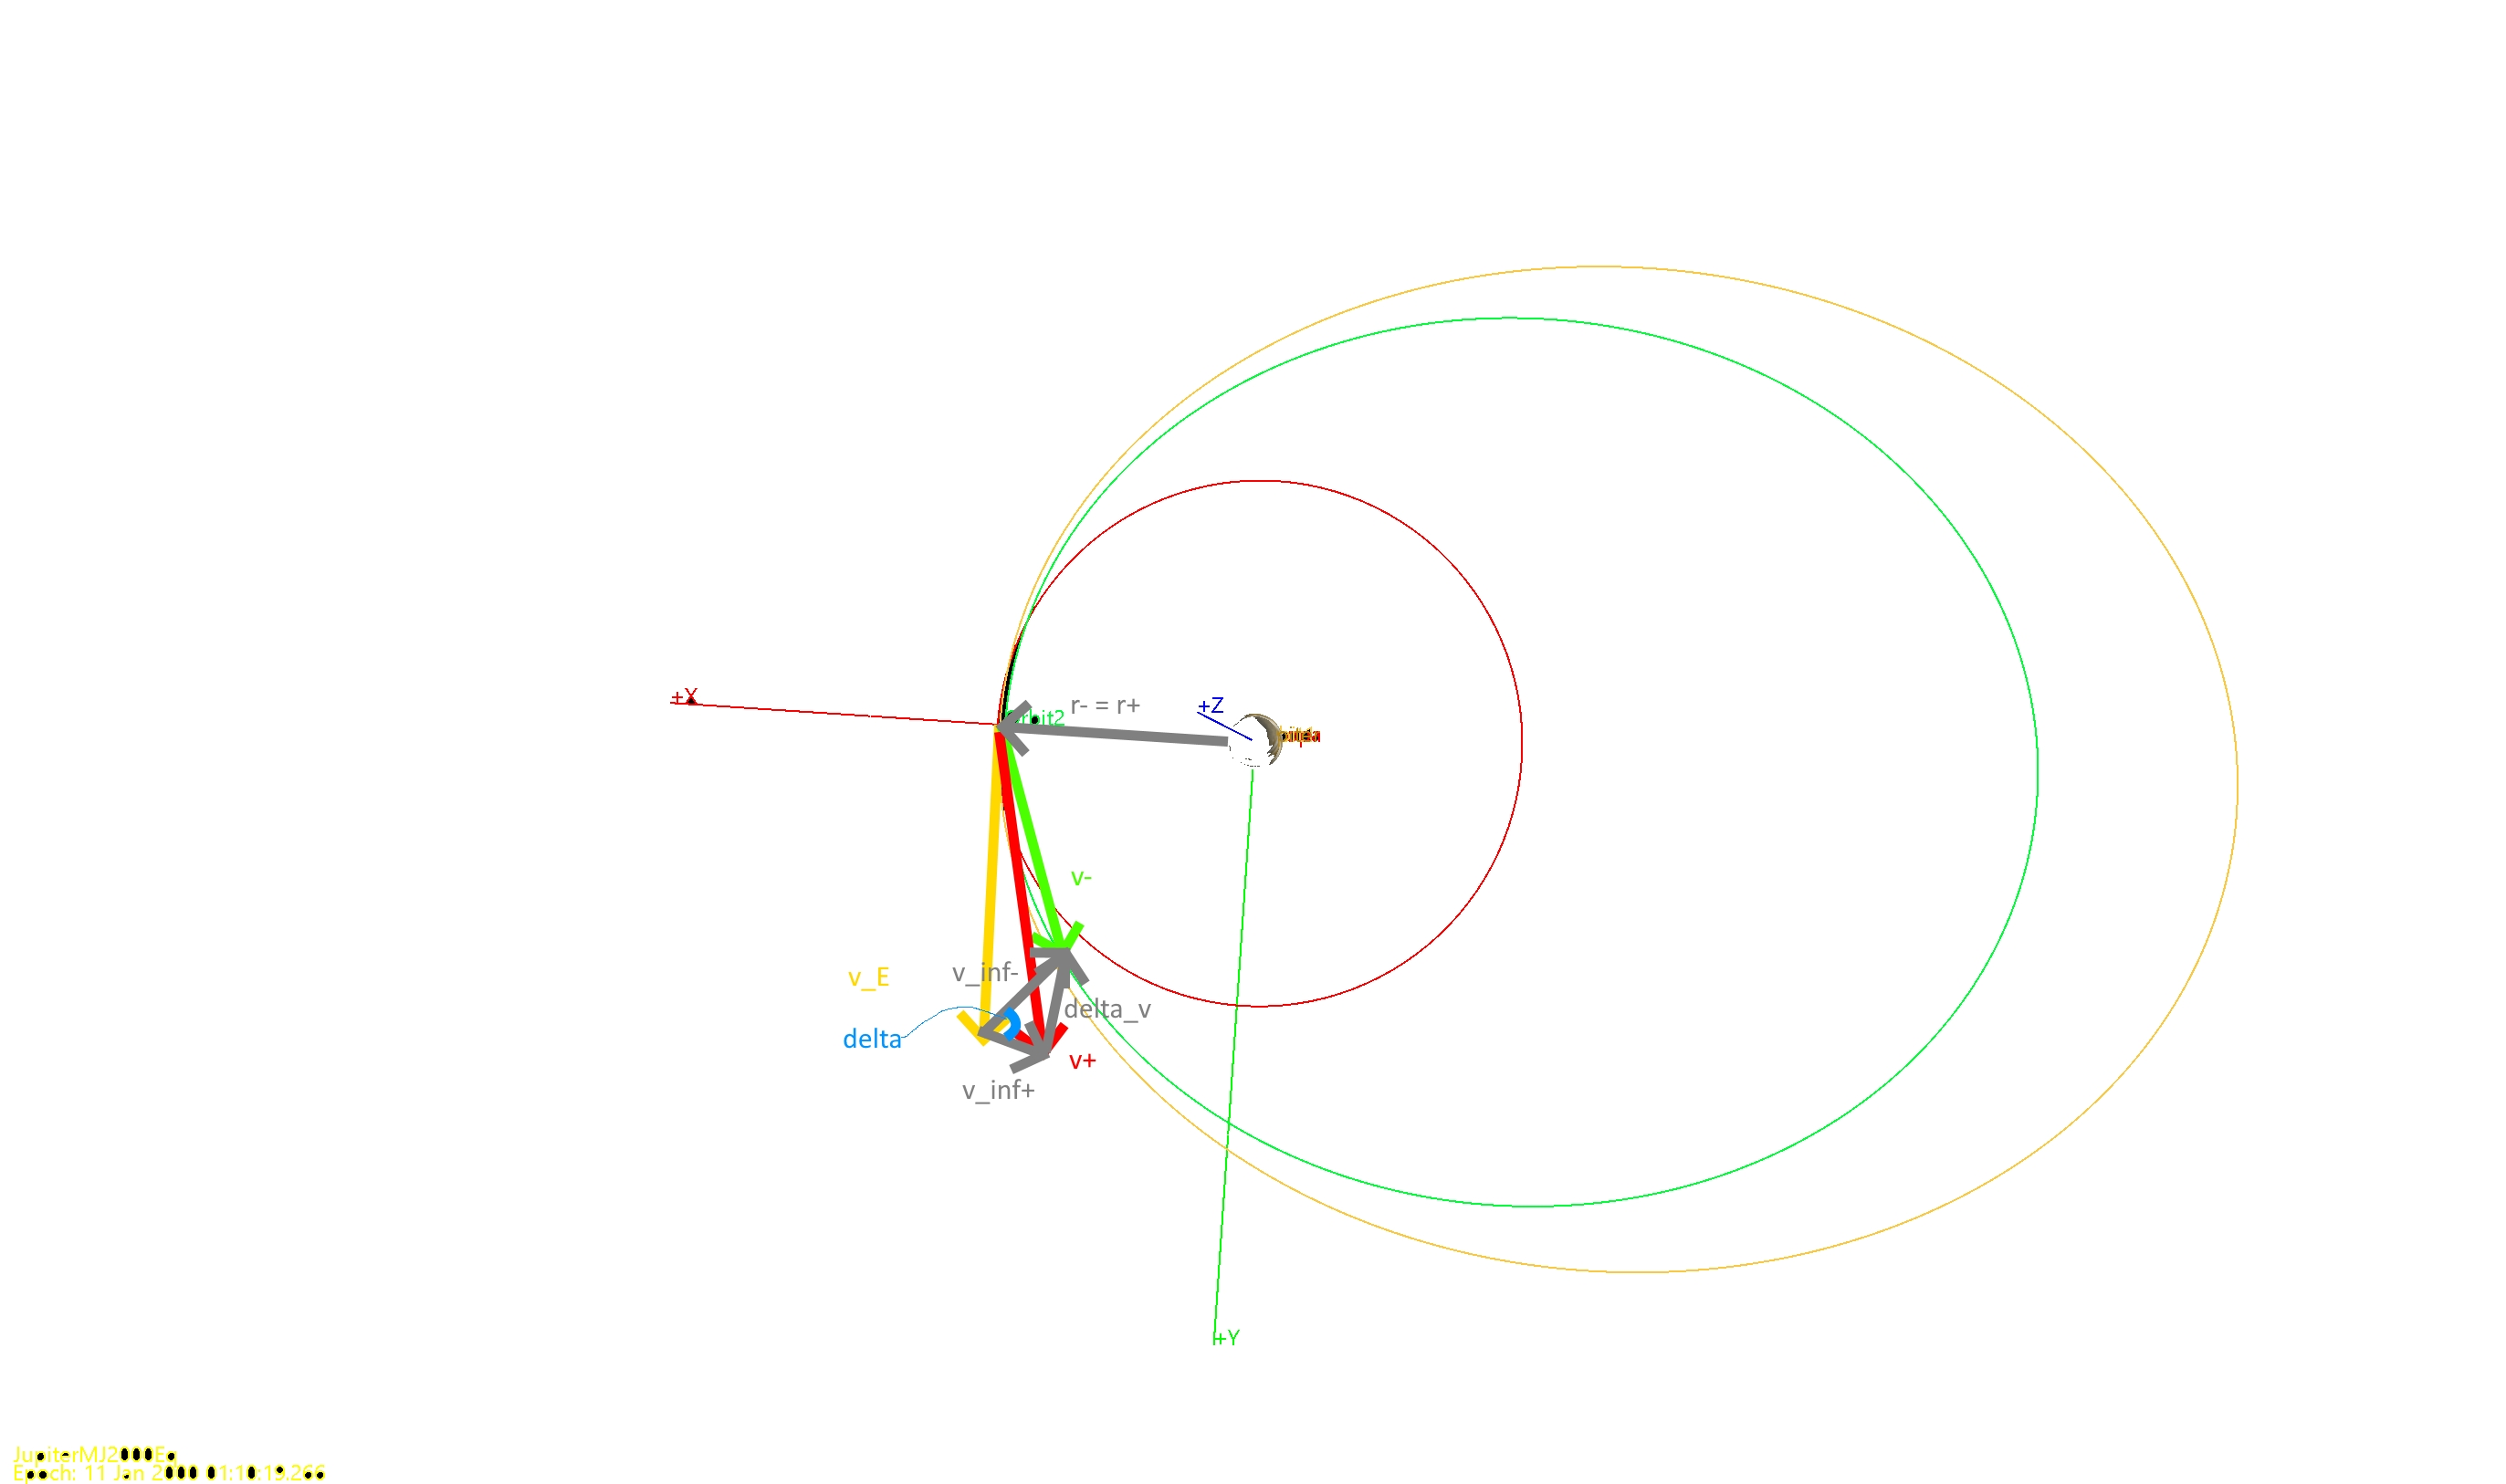
\includegraphics[scale=0.2]{diagram}
  \caption{GMAT with orbital properties}
  \label{fig:Fig1}
\end{figure}
\begin{figure}[!htb]
  \center
  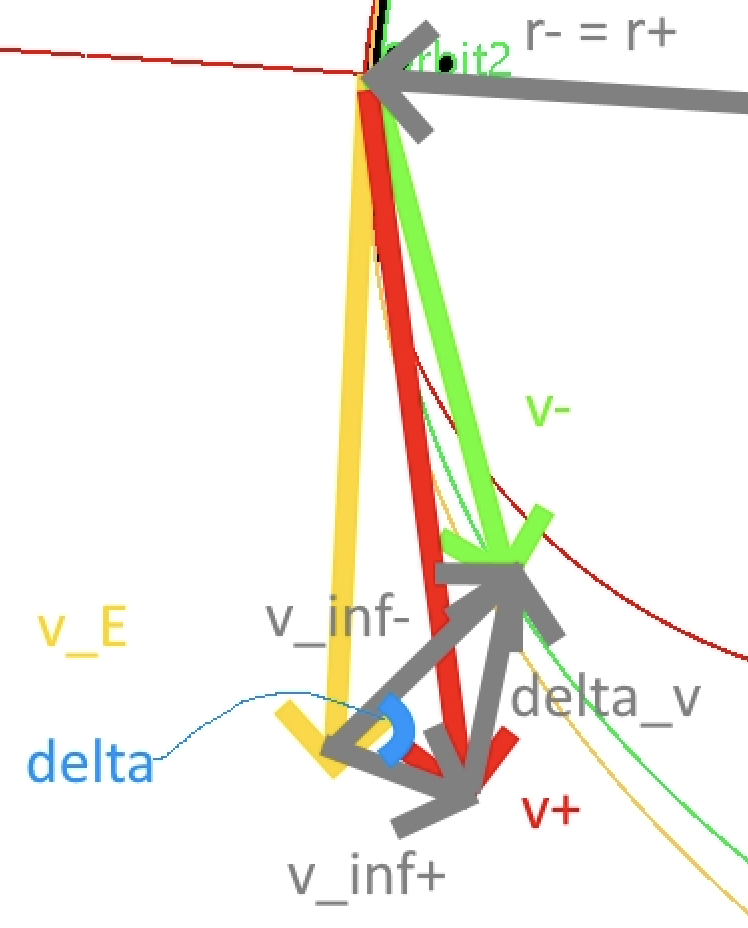
\includegraphics[scale=0.5]{detail}
  \caption{Detailed View}
  \label{fig:Fig2}
\end{figure}

\vspace{10px}
\newpage
8. Clipper's mission could involve over 45 fly-bys of Europa. If the goal is to return to Europa, would you have the spacecraft perform the fly by?\\
I would not have the spacecraft perform this fly-by. The radius of clipper at periapsis around Europa is 1359km while the radius of Europa is 1561km. This is an impact trajectory. Another path would need to be chosen to avoid clipper impact with Europa.
\newpage
HW5.m
\begin{lstlisting}[frame=lines,style=Matlab-editor,basicstyle = \mlttfamily]
clc; clear all; close all

%constants
MU = 42828;

% Problem 1
vr = [-2089.6 -2515.7 -6382.0];
vv = [2.1744 0.76911 0.13452];

r = norm(vr)
v = norm(vv)

vh = cross(vr, vv);
h = norm(vh);

syms a
energy_eqn = v^2/2 - MU/r == -MU/(2*a)
energy = v^2/2 - MU/r
a = double(solve(energy_eqn, a))

syms e
h_eqn = h == sqrt(MU*a*(1-e^2))
e = double(solve(h_eqn,e))
e = max(e)

syms E
E_eqn = r == a*(1-e*cos(E));
E = double(solve(E_eqn,E));
E = -min(E) %Because it is descending.

syms time_since_p
time_since_p_eqn = sqrt(MU/a^3)*time_since_p == E - e*sin(E);
time_since_p = double(solve(time_since_p_eqn,time_since_p))

% Problem 2
p = h^2/MU;
true_a = -acos(p/(r*e) - 1/e)
vv_rt = [h*e/p*sin(true_a) h/r 0] % answer

% Problem 3
E1 = E;
t1 = time_since_p;
vr1 = vr;
vv1 = vv;
r1 = r;
v1 = v;
t2 = time_since_p + 12*60*60;
n = sqrt(MU/a^3);
M = n*t2;
E2 = fzero(@(x) x-e*sin(x)-M, 0);
f = 1 - a/r*(1-cos(E2-E1));
g = (t2 - t1) - sqrt(a^3/MU)*(E2 - E1 - sin(E2 - E1));

vr2 = f*vr + g*vv;
r2 = norm(vr2);
fdot = -sqrt(MU*a)/(r2*r1)*sin(E2-E1);
gdot = 1 - a/r2*(1-cos(E2-E1));

vv2 = fdot*vr1 + gdot*vv1 % intertial unit vectors

true_a2 = -acos(p/(r2*e) - 1/e)

vv2_rt = [h*e/p*sin(true_a2) h/r2 0] % radial-tangential

% Problem 4
vr2_peri = [r2*cos(true_a2) r2*sin(true_a2) 0]
vv2_peri = sqrt(MU/p)*[-sin(true_a2) e+cos(true_a2) 0]

% Problem 5

% find i theta omega
syms inc
h_hat = cross(vr2, vv2)/norm(cross(vr2, vv2))
inc_eqn = cos(inc) == dot(h_hat, [0 0 1])
inc = double(solve(inc_eqn,inc))
inc = max(inc)

syms RAAN
RAAN_eqn_1 = sin(RAAN)*sin(inc) == dot(h_hat, [1 0 0])
RAAN_eqn_2 = -cos(RAAN)*sin(inc) == dot(h_hat, [0 1 0])
RAAN1 = double(solve(RAAN_eqn_1));
RAAN2 = double(solve(RAAN_eqn_2));
RAAN = min(RAAN1)*180/pi

syms arg_peri
r1_hat = vr1/norm(vr1)
theta_hat = cross(r1_hat, h_hat)/norm(cross(r1_hat, h_hat))
syms theta
theta_eqn_1 = sin(inc) * sin(theta) == dot(r1_hat, [0 0 1])
theta_eqn_2 = sin(inc) * cos(theta) == dot(theta_hat, [0 0 1])
theta1 = double(solve(theta_eqn_1, theta))
theta2 = double(solve(theta_eqn_2, theta))
theta = intersect(theta1, theta2)
arg_peri_eqn = arg_peri == theta - true_a
arg_peri = double(solve(arg_peri_eqn, arg_peri))
\end{lstlisting}

\end{document}
